% vim: set tw=78 sts=2 sw=2 ts=8 aw et ai:

\chapter{Current deployment}\label{ch:current}
\bigskip

\section{UDPCast}


Setting up a computer means two things: getting the hardware (a normal
PC) and installing a modern Operating System on it to control that
hardware. This is a job that would take a normal person, with basic
computer operating skills, about one hour on average. However, the
normal approach does not scale to installing on 3 or more hosts that
need the exact same setup.


In office environments, Internet/Game Cafes and, most important, in
school laboratories where 15 to 20 computers with identical
configuration need to be set up, an imaging solution is needed.  This
means that the setup will be done on a single computer and then, the
entire disk on which the new operating system resides is copied
throughout the network onto the disks of the other uninstalled hosts.
This can save, for a number of 20 hosts, from 20 hours of work to only
two hours (about one hour for installing one system and another hour
for the copy of the disk(s) over the network).


To get a perfect mirroring, it is recommended that the hosts be
identical (same CPU, same Main board, same \ac{HDD}s, same network card).
If the systems differ in a slight way, it is up to the operating
system to try and adapt to new hardware and install the appropriate
drivers.  From the operating system’s point of view, it is like the
HDD was taken out of one computer and installed in another one.

\begin{figure}[h]
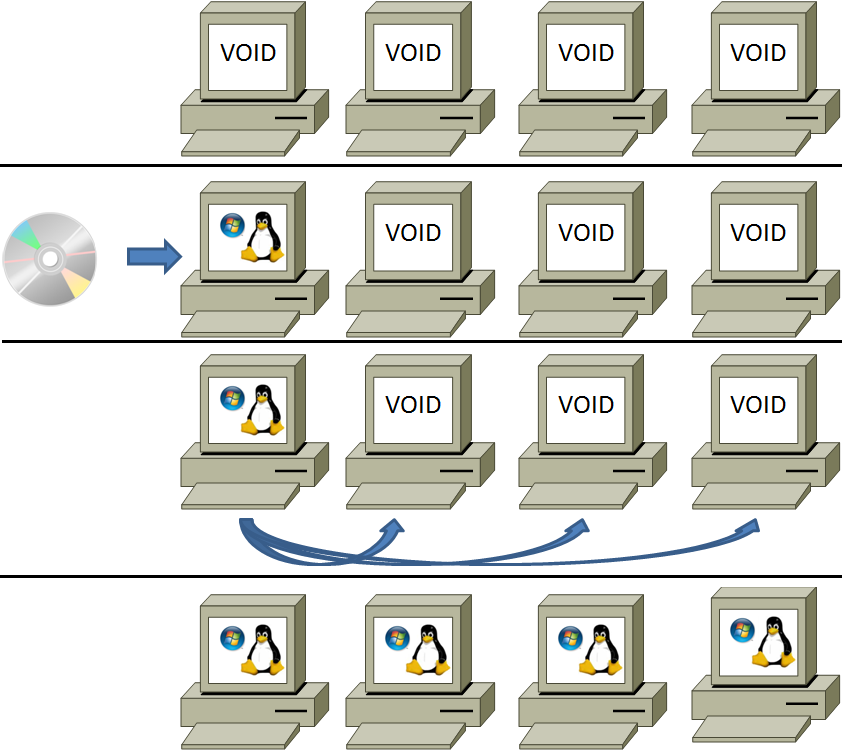
\includegraphics[width=10cm]{img/4comp}
\caption{Simple imaging operations}
\label{fig:4comp}
\end{figure}


To image a network of stations, there are some basic steps you need to take

\begin{enumerate}
\setcounter{enumi}{0}
\item Prepare all the hosts so they can power on. They can have empty
hard disks or hard disks with data that can be deleted.


\item Install one or more operating systems on one host.  This host will
be the seed host.  The operating system(s) can be personalized with
user accounts, installed programs, configured environments. Along with
the operating system(s), on the hard disk there will be the stage 1
boot loader in the \ac{MBR} and the upper stages of the boot loader on
other partitions. Separate partitions for personal data or backups can
be created


\item All the hosts must be able to boot in a pseudo-operating system
provided by the imaging software from a Live CD,  over the network via
PXE or from a local special partition so the working operating is not
modified during the imaging operation.


\item The contents of the seed’s hard disk are copied over the network
(usually using UDP over Multicast IP).  After the transfer is
complete, all hosts boot up normally.
\end{enumerate}



When using imaging systems, software licensing must be taken under
consideration.  The software that has per host or per CPU license has
to have a separate license code for each host.
There are two widely used software suits that provide system imaging:
Symatec Norton Ghost and UDP Cast. The first one is a professional
closed source enterprise software while the second one is an open
source project developed by a community.  Because of the flexibility
of open source projects, UDP cast, has been used in the development of
this imaging system solution and will be described in more detail.

UDP Cast is an open source project that offers a file transfer tool
that can send data simultaneously to many destinations on a \ac{LAN}, under
the \ac{GPL} 2.0 License. The program, along with its source code can be
downloaded from their site, at http://udpcast.linux.lu/.
The compiled projects, offers two executables:  udp-sender and
udp-receiver. By default, the two programs can be used to send input
from standard input on the sever side to all the clients which print
the received data to standard output.


On top of the two executables (udp-sender and udp-receiver) the UDP Cast
Project offers a Live CD (that can be found on their website) built to run
a wizard for the configuration for a sender or a receiver of a system
image. The iso file can be burned onto a CD or set up on a PXE network
boot.

The Live CD is a Linux Distribution based on Debian, stripped down to
occupy a small amount of memory and boot very fast. It must be booted on
all workstations that will participate in the imaging process (the seed
that is the sender and all the receivers)

After the kernel loads, it must load kernel modules (device drivers)
for the \ac{NIC} and the hard disk drives.


When the \ac{OS} has loaded the device driver, it can configure
network connectivity. This is done either by setting up a manual IP address
with a valid subnet mask or by use of \ac{DHCP} automatic configuration.
Obtaining an IP address is mandatory for the system to work because,
without an IP, the sender can't connect to the receivers.



After the device driver for the hard disks (PATA, SATA, SCSI) is loaded,
the user must chose what partition or device will be imaged. This has local
significance. On the seed host it will be the partition that will be sent over
the network and on the receivers it will be the partition on which the data
will be written. The name of the partitions are Linux formated. The user
can select a single primary or logical partition (ex. hda1, sda2, sdb5) or
an entire drive (hda, hdb, sda). The \ac{MBR} is found on the first 512bytes of
the physical drive.

It is recommended that the same option be selected on all devices.



A partition is usually has a very large data size and the transfer over the
network could be time consuming. For computers with good enough processing
power, compression can be used. UDP Cast offers two types of compression
\begin{itemize}
\item \ac{LZOP}
\item \ac{GZIP}
\end{itemize}

The use of compression can reduce the sent data by a factor of up to 50\%.


After all the configurations are made (they should be identical in most
conditions), the direction of the transfer must be specified on each host.
One workstation will be the sender and all the others will be the
receivers.


A proposed optimisation of using the UDPCast in laboratory environment
has been discussed in a previous thesis that I authored \cite{paper:me}.
It presents a centralized approach using a Python based client-server
architecture. While this creates a central node that stores a database
of operating system images, it cannot control the other nodes remotely.
This is a pull model where the administrator has to visit each node and
configure it to ask for an image from the server.

The centralized architecture has the big drawback of making the
administrator physically move between stations to complete the work.

Another problem with that approach is the fact that the client-server
protocol proposed is in a very early stage of development so it is not
an industry standard.

Some of these problems could be resolved given a proper remote
management system.

\section{Freezing script}

The freezing script has been developed by Mircea Bardac and Geroge
Milescu from the Computer Science Department at UPB. The central part of
it is the \ac{AUFS} filesystem that is used an intermediary layer for
the operating system's root file system. This script is made for Linux
distributions.

A normal boot of a Linux distribution has its root filesystem hierarchy
can be mounted from one or several partitions. Those mountpoints are
usually in read-write mode. With the exception of mountpoints such as
/proc and /dev that use the procfs and devfs filesystems, any \ac{IO}
results will results in changes on the physical partition.

The \ac{AUFS} mountpoints act as an extra layer in the IO operations
stack.The freezing script requires an extra partition reserved on the
hard drive (or a large file, like a swapfile). The \ac{IO} operations
will be done in the Linux \ac{VFS} are done as usual, but are
intercepted the \ac{AUFS} and the changes aren't pushed on the physical
device, but wrote in the special freezing partition.

While the system is running, the freezing partition is used in a
\ac{COW} mode: when files are needed from the root partition, they are
copied to the freezed partition and used from there. At a reboot, the
freezing partition changes are ignored and the files from the root
partition(s).

For Windows systems, a similar, enterprise and closed source product is
available: \emph{DeepFreeze}.

The architecture of the system gives an inherited flaw: the latency
caused by sometimes needing to double copy. If large files are involved,
the latency is visible to the user.


\begin{table}
\begin{tabular}{|p{4cm}|p{3cm}|p{3cm}|}
\hline
Action & Time on no-freezed syste & Time on freezed system \\
\hline
Write 1GB file from /dev/zero & 6.7s & 6.7s \\
\hline
Reading newly created file (1GB) & 1.4s & 1.5s \\
\hline
Reading file from root system (1GB) & 1.4s & 8.1s \\
\hline
\end{tabular}
\caption{Latency when using freezing system}
\label{table:aufs_latency}
\end{table}

As seen in table \ref{table:aufs_latency}, writing or reading new files
has no impact on IO times because the operations do a single write (one
to the root partition directly one to the freezing partition, directly).
But when you access a file that exists on the root partition, it first
needs to copy the file from the root partition to the freeze partition,
and that could take as much as 5 times more time.

A new approach for a freezing system with support in the Linux kernel
has been discussed in another thesis \cite{paper:freezing}.

\section{Virtual machines}


Virtual machines have become essential in computer laboratory rooms.
They provide easy to setup and deploy environments.

A thorough presentation of what virtualization is, what are the current
available technologies and what is their role in education is covered by
Huber et al. \cite{paper:virtualization}. The term virtualization refers
to any abstraction of a physical system and its resources from
asoftware. The virtualization can be for an application, a process or an
entire operating system. The main purpose of a virtualized environment
is to provide a layer of security by containing the guest system from
interacting with the main hardware or the resources from another guest.

There are a number of types of virtualization, each with its own
approach and its use-case.

\emph{Virtual memory} is one of the first ways of virtualizing hardware.
Rather than each process of an operating system having access to the
main physical memory, it has access only to its own virtual memory This
secures one process from all other processes on the system and gives
each process the same amount of memory, regardless of the actual
physical memory, offering portability of the process code. The
operations on the virtual memory is supervised by the operating system
and uses the \emph{ MMU (Memory Management Unit)} that needs hardware
support.

\emph{Emulators} hide the real hardware from a guest by rewriting every
hardware operationin software. A virtualized process or operating system
would run inside a process in the host’s operating system. Any
architecture can be emulated in software but at a high loss of
performance. QEMU, Dynamips or DosBox are examples of emulators.

\emph{Paravirtualization} uses a hypervisor to trap operations from a
guest machine and makes decisions on weather to resolve them by itself
or to send them to the actual hardware to be resolved. Xen is a
paravirtualization solution.

\emph{Hardware-assisted virtualization} is a form of full
virtualization, in which the hardware is aware of the fact that programs
are running in a container.Full virtualization can only work if the
processor has hardware support for virtualized operations.  Instructions
run directly on the hardware, without intervention from a hypervisor.
VMWare Workstationand and  Virtual Box use this kind of virtualization.
KVM is built specifically to handle this kind of virtualization.

\emph{Operating system level virtualization} is done within a modified
Operating system. The kernel is shared by all the virtual machines,
including the host node, but only the processes in the same virtual
machine, called a container, can interact with each other.  OpenVZ and
LXC are the implementations of this type of virtualization.

Each solution has its strengths and weaknesses. Some solutions are more
suitable than others in different conditions. For example, emulators are
slow, but they can offer more virtualized architectures to the guest
machine. Paravirtualization needs the guest operating system to be
modified to work. Full virtualization requires hardware support but is
very efficient. Operating system virtualization are lightweight but a
crash to in the kernel of one virtual machine means the crash of all
machines because of the shared kernel.


The current deployment at UPB involves using several of these
technologies. VMware Player (or VMware Workstation) and its open
equivalent, Virtual Box is used in labs where full virtual machines need
to be deployed.

They provide an user friendly and intuitive interface
for students to use and have many many features to offer. One important
feature is the \emph{Snapshot} of a virtual machine. A student can store
the exact state of a virtual machine (both disk state and RAM state),
continue to use the virtual machine, and then revert back to the
snapshot state. This a much more efficient approach compared to saving
an archive of the entire machine and recovering the initial state from
that backup, because a snapshot only saves the differences from the
initial state.

But solutions like VMware Workstation/Player or Virtual Box require
more strict hardware resources. Workstations with hardware
virtualization support provide a much better infrastructure. If such
support is available, \emph{\ac{KVM}} is a better solutions, scaling
to more virtual machines per host (an experiment regarding this will be
covered later).

OpenVZ or LXC provide more containers per physical node than other
virtualization solutions. It can be used of lightweight deployments.
Since more containers can be deployed per node, more advanced topologies
can be installed using virtual networks.

No matter what solution is chosen, the deployment of new machines (new
topologies or new versions of same topologies) is dependent on an
UDPcast of the workstations.

Moreover, in the case of solutions such as KVM or VMware, because of the
large files that store the virtual disks, opening the machines take a
big latency hit because of the freezing system.
